\inputencoding{utf8}
\chapter[Testiranje zmogljivosti Amazon EC2 platforme (P. Matičič, J. Pelicon, B. Rojc)]{Testiranje zmogljivosti Amazon EC2 platforme}

\pagestyle{fancy}
\fancyhf{}
\fancyhead[LE,RO]{\thepage}
\fancyhead[RE,LO]{\leftmark}

\huge Peter Matičič, Jan Pelicon, Blaž Rojc
\normalsize
\bigskip

\section{Opis problema}

Z dneva v dan proizvedemo čedalje več slik.
Predstavljajo znaten delež podatkov, shranjenih v raznih storitvah v oblaku.
Ampak ko želimo najti določen predmet ali osebo, ki smo jo slikali, je ročno brskanje po digitalnih zbirkah zamudno.

S tem problemom v mislih bomo stestirali oblačno platformo Amazon EC2.
Ustvarili bomo enostavno storitev, ki bo uporabniku omogočala iskanje vzorcev v večjem naboru slik, shranjenih v oblaku.
Poglobili se bomo v zahtevnost uporabe za programerja, fleksibilnost pri programiranju in morebitnem prenašanju storitve na druge platforme,
	odzivnost in izkušnjo za uporabnika ter zmogljivost in skalabilnost virov na platformi.
	
	\begin{figure}[H]
    \centering
    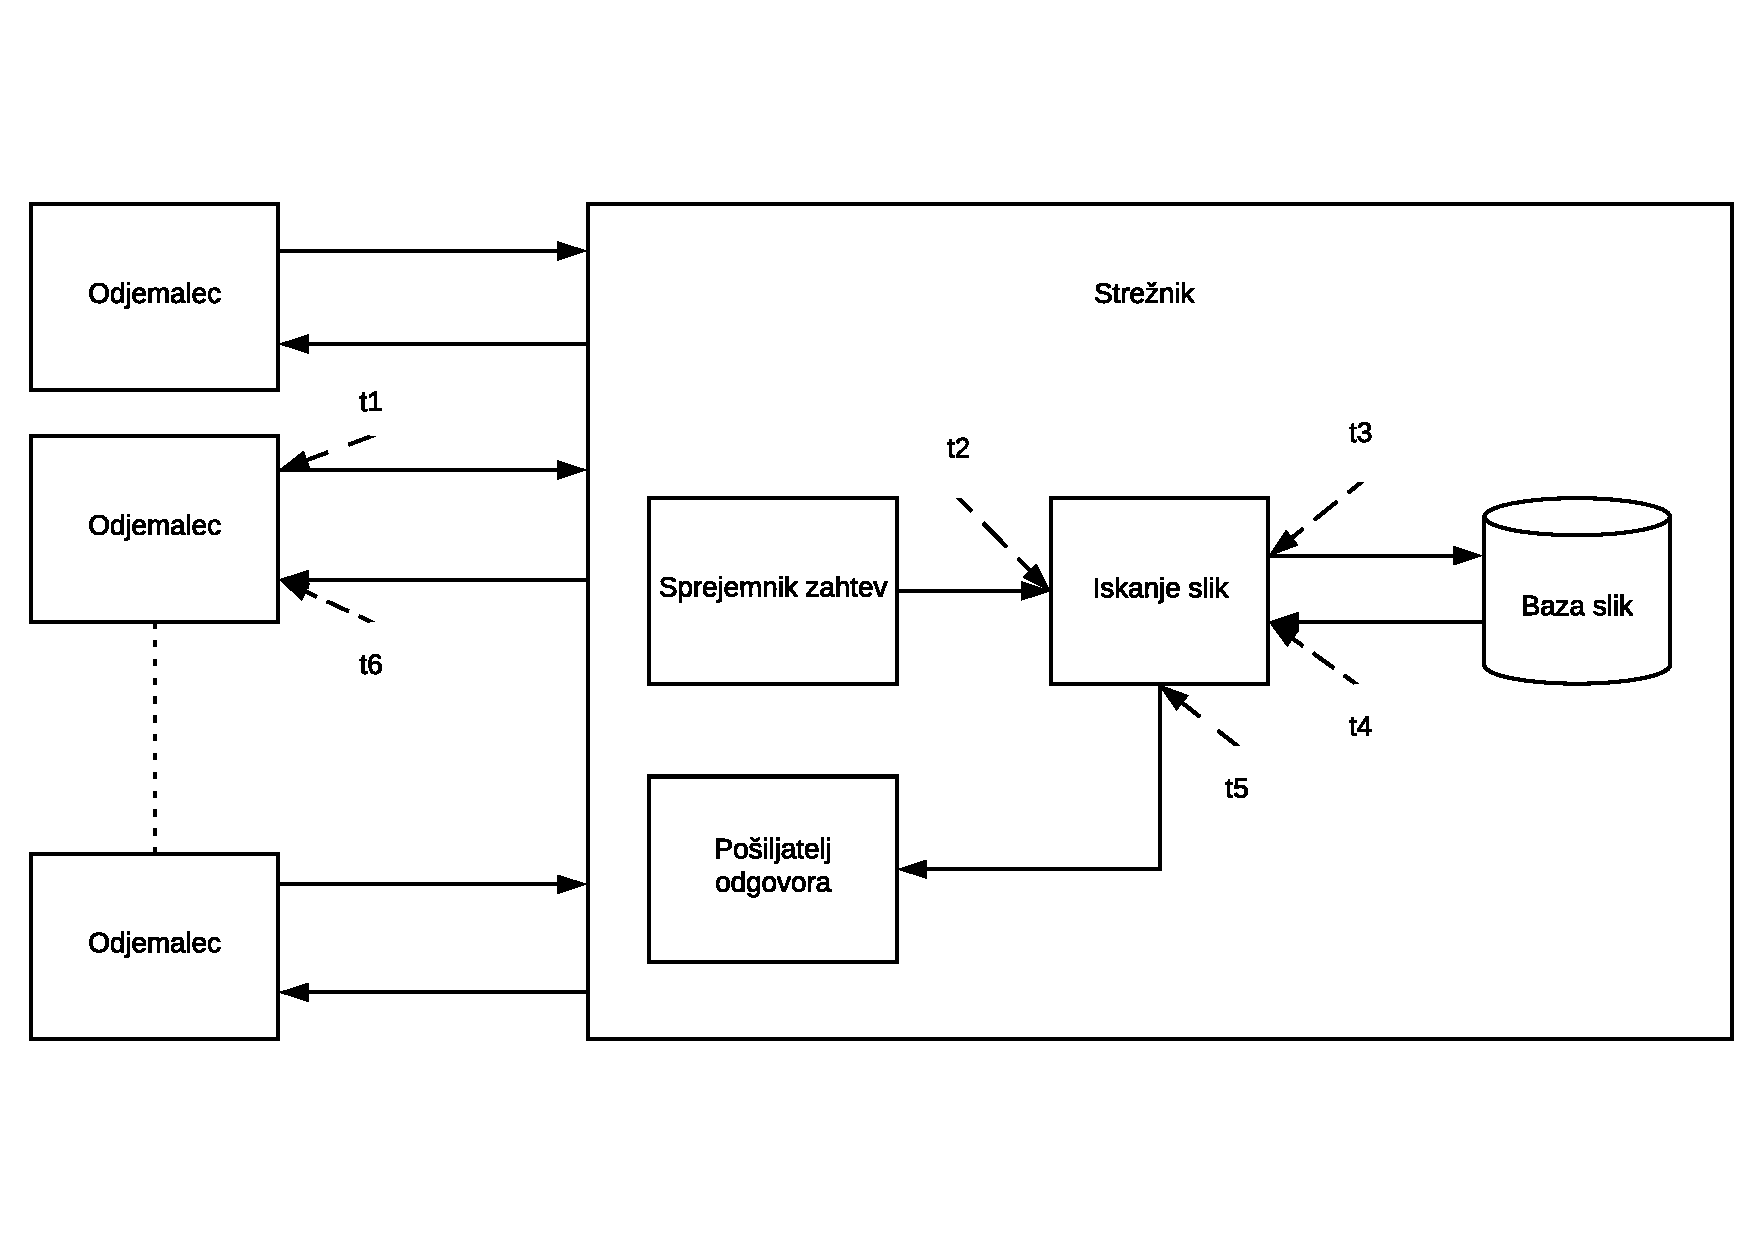
\includegraphics[scale=0.4]{Img/1_shema.pdf}
    \caption{Shema aplikacije.}
    \label{fig:1_osnovnaShema}
\end{figure}

\section{Realizacija}

\subsection{Način iskanja vzorca}
\begin{itemize}
\item Iskanje ene slikovne točke v množici slik ki bo ustrezala zahtevam.
\item Iskanje vzorca podanega z masko v mnžici slik.
\item Iskanje slike, ki vsebuje podan slikovni izsek.
\end{itemize}

\subsection{Amazon AWS račun}

\subsection{Aplikacija}
Aplikacija bo narejena v jeziku Java. Na strani pošiljatelja bomo generirali zahteve in jih pošiljali na strežnik v obliki JSON. Strežnik bo lahko hkrati obdeloval več zahtev do mere ki mu bo omogočal dostop do slik.


\section{Predvidevanje metrik}
Kot glavno metriko bomo opazovali skupni čas zahteve in odgovora. Podrobneje ga bomo razdelili na čas potovanja zahteve od nas do strežnika, čas obdelave na strežniku in čas potovanja odgovora od strežnika do nas.

\section{Rezultati meritev}

\section{Plan dela}
\begin{itemize}
\item snovanje ogrodja storitve
\item določitev bremen
\item določitev metrik
\item določitev orodij
\end{itemize}

\section{Literatura}

\inputencoding{cp1250}